\section{Motivation}\label{sec:intro}
The aim of this report is to investigate the dynamics of motion of a  helicopter, then develop suitable models to control it, and furthermore, refine and implement them in MATLAB to get the best control that we can manage. The theoretical background for this analysis is the  curriculum of the course "Linear system theory", TTK4115. The lab took place over 8 weeks in the fall of 2017 at NTNU.

The report, and assignments, are structured into multiple sections. \Cref{sec:part1} develops the dynamics of the helicopter by examining the torque at the joint angles, \textit{p, e, $\lambda$}, and from that constructing differential equations relating the angles to the voltage applied to the helicopter rotors. From there we linearize our model and do a similarity transform to get a system of equations that we can apply our linear system theory too. In \Cref{sec:part2} we apply mono-variable control to control the pitch and travel of our helicopter. In \Cref{sec:part3} we examine the multi-variable system and apply optimal control. The last part of the assignment, \Cref{sec:part4}, we introduce an observer to our system to suppress noise and perform state estimation. The last section, \Cref{sec:conclusion}, is a final evaluation of our methods and results.

\subsection{Lab setup and model of helicopter}
A force diagram illustrating the forces acting on our helicopter is shown in \Cref{fig:heli}, which is available here \cite{github}. The helicopter has two rotors providing thrust, that rotate around the pitch-axis, \textit{p}. The weight of these rotors are then counteracted by a counterweight and can rotate around the elevation-axis, \textit{e}. And this system can then rotate around the travel-axis, $\lambda$.

The helicopter is connected to a workstation PC so that it can be software controlled using MATLAB and Simulink. The joint angles are measured using a radial encoder at each joint, and the measurements are sent over to the workstation. A joystick is also connected to the workstation, and is used to set the reference points for our various controllers throughout this assignment.

\begin{figure}[tp]
	\centering
	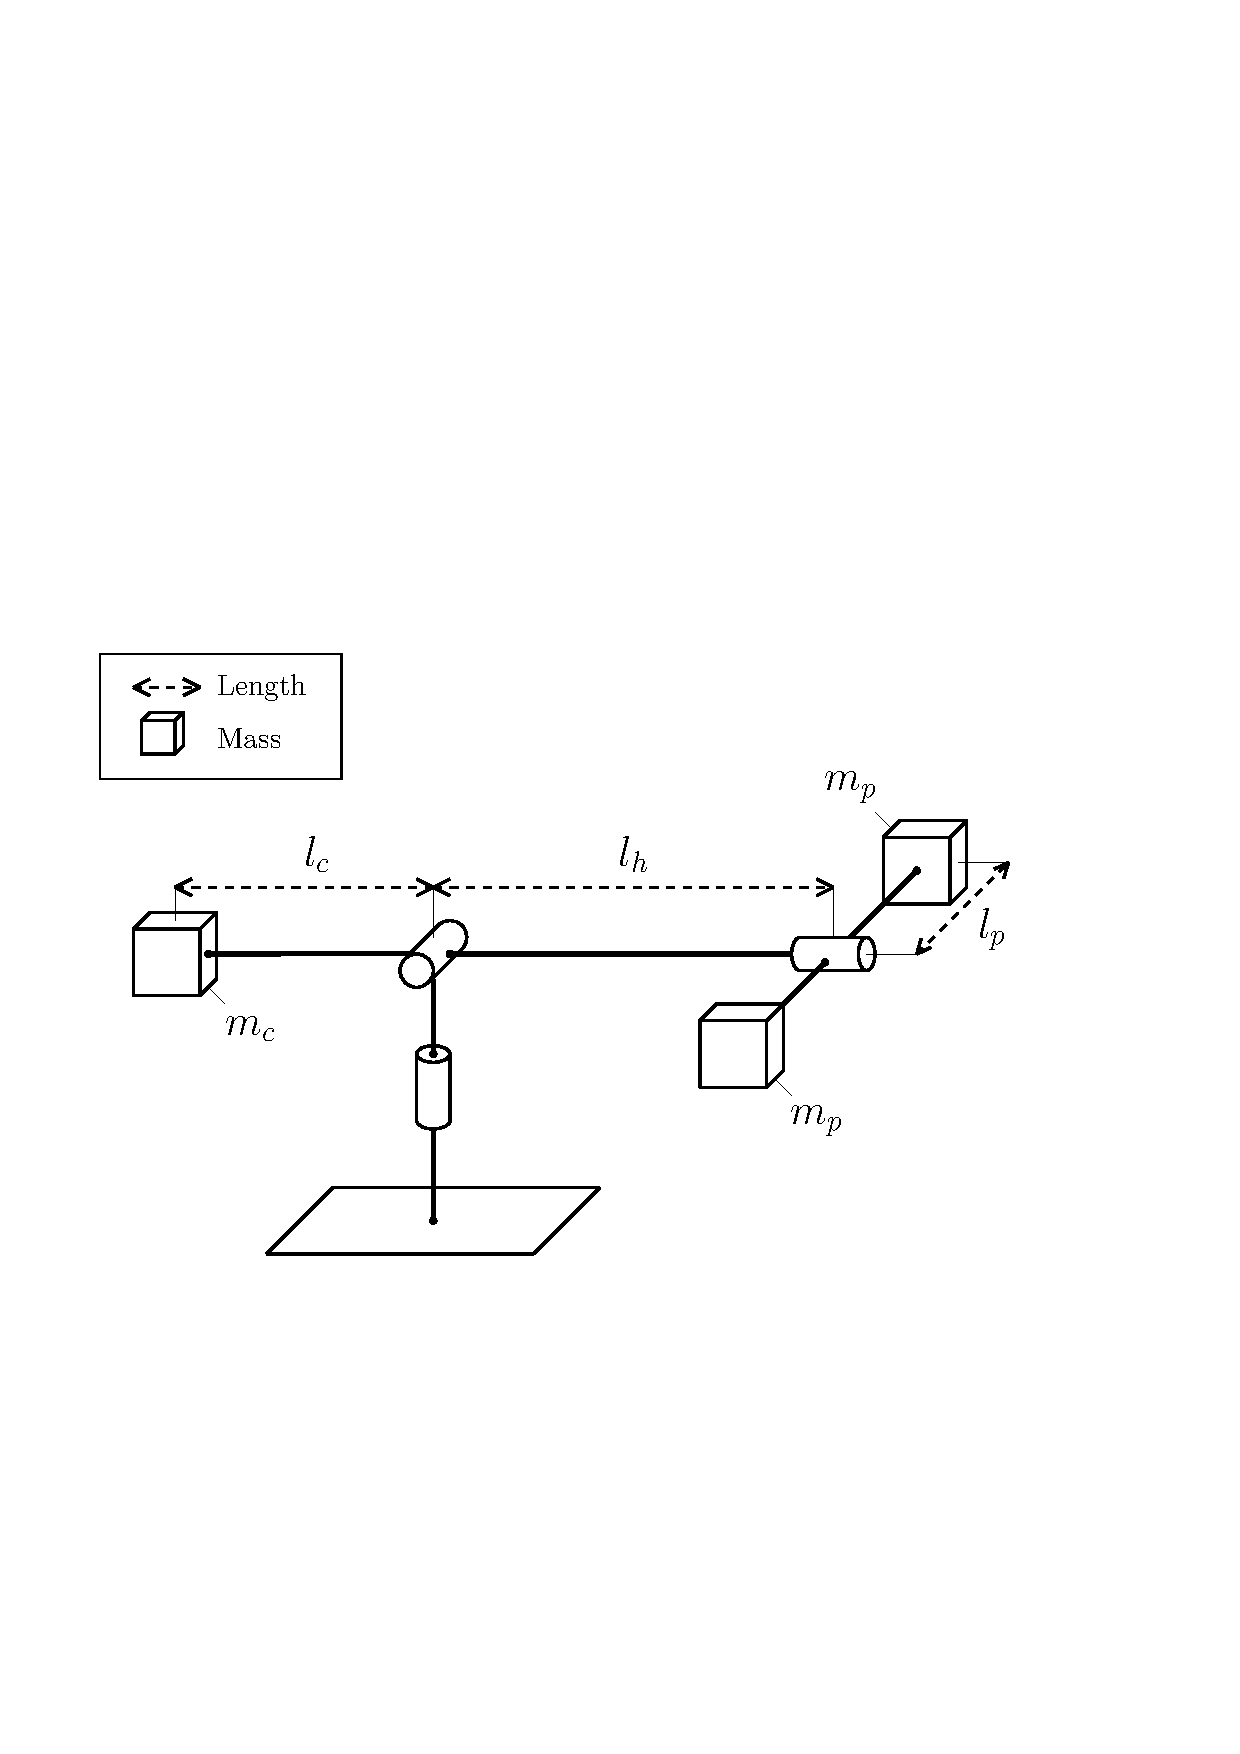
\includegraphics[width=1.00\textwidth]{figures/masses.pdf}
	\caption{Masses and dimensions of our helicopter.}
\label{fig:masses}
\end{figure}

\begin{figure}[tp]
	\centering
	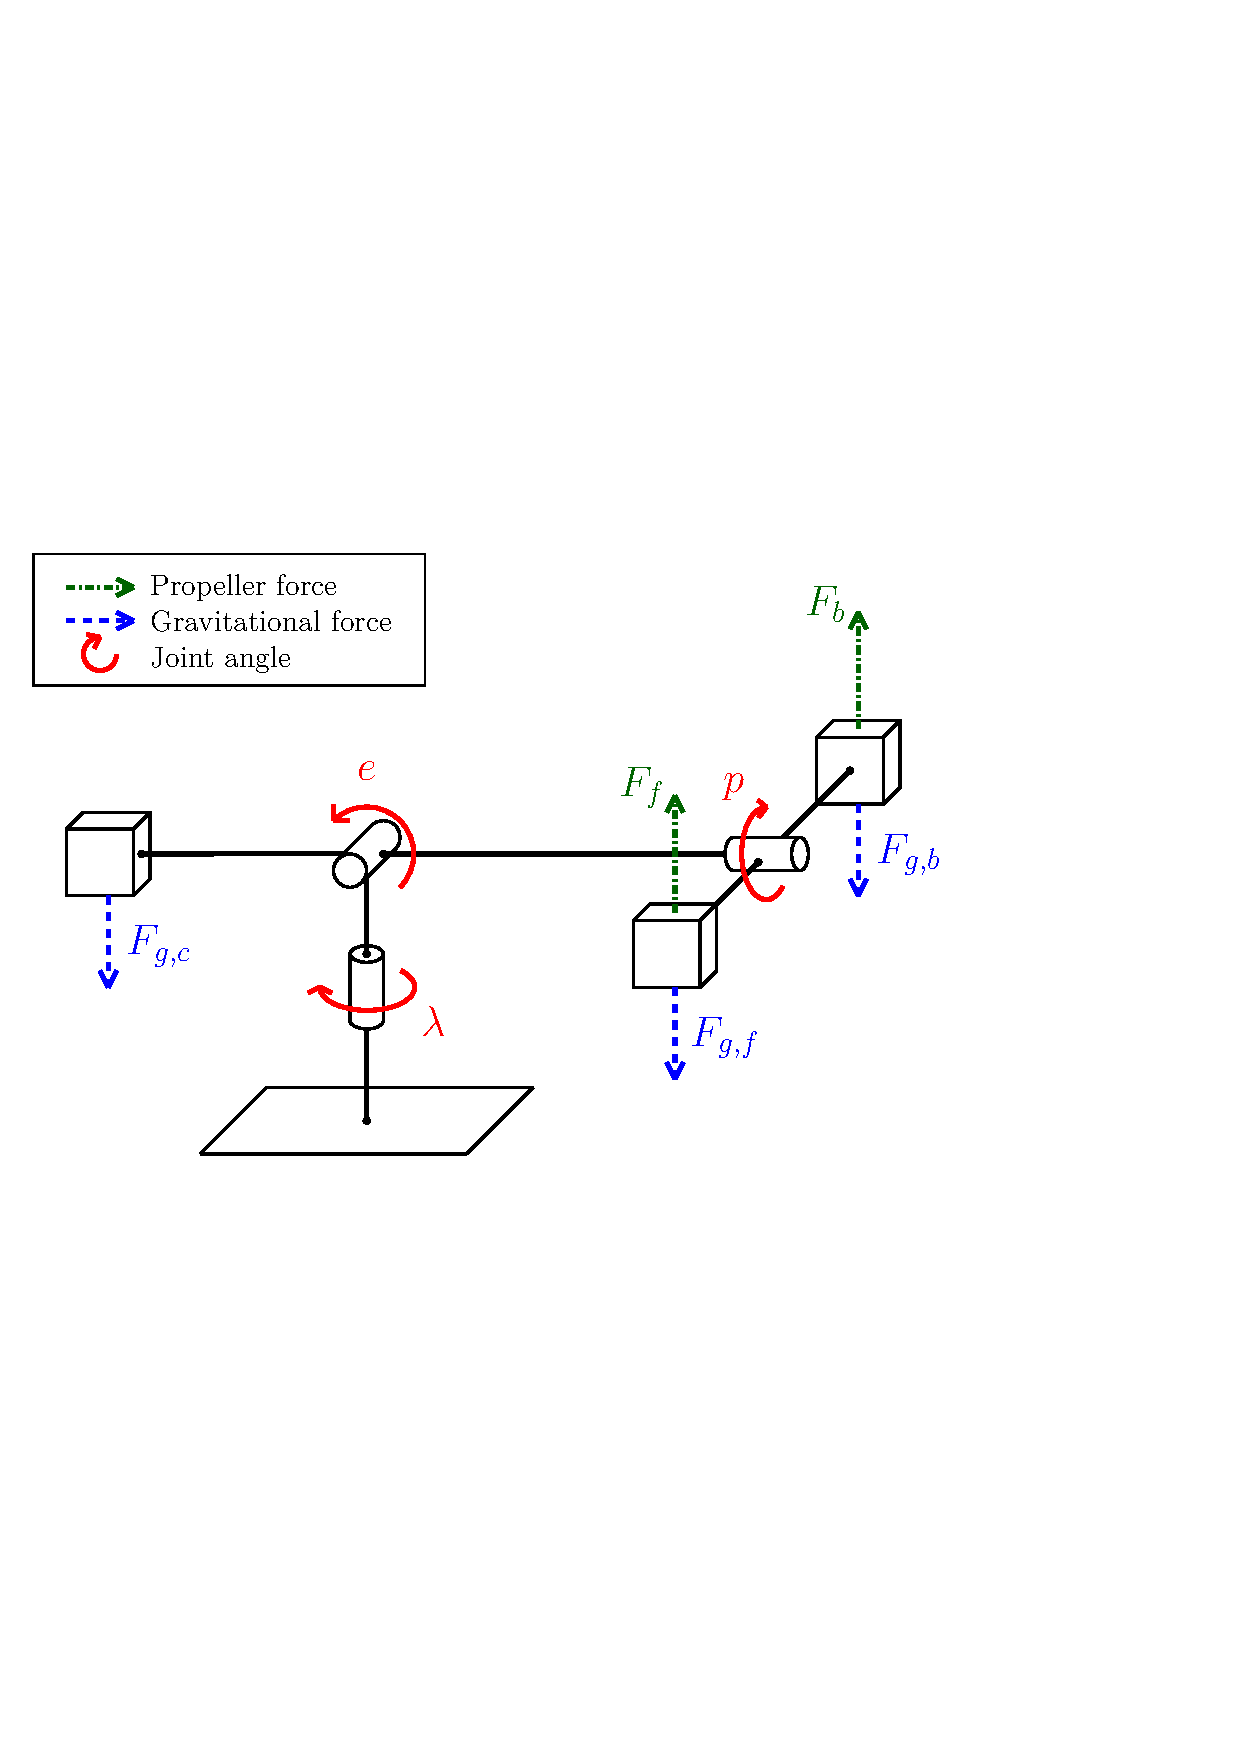
\includegraphics[width=1.00\textwidth]{figures/forces.pdf}
	\caption{Force diagram representation of our helicopter.}
\label{fig:heli}
\end{figure}

